\chapter{Fundamentação Teórica}
\label{chp:ass}

Este capítulo estabelece a base conceitual para a proposta metodológica do Capítulo~\ref{chp:capitulo4}: parte das etapas de pré-processamento e avaliação de modelos de aprendizado de máquina (Seção~\ref{sec:treinamento-ml}), avança para o paradigma de aprendizado de máquina informado por física e a formulação de PINNs (Seção~\ref{sec:des2}), caracteriza fisico-quimicamente o processo BOF (Seção~\ref{sec:des3}), e encerra discutindo geração de dados sintéticos, interpretabilidade via SHAP e arquiteturas híbridas físico-informadas (Seções~\ref{sec:dados-sinteticos-fund}--\ref{sec:arquiteturas-hibridas}).

\section{Treinamento de Modelos de Aprendizado de Máquina}
\label{sec:treinamento-ml}

Esta seção aborda as etapas preparatórias intrínsecas a treinamentos eficazes
de modelos de aprendizado de máquina. Inicia com a exploração das práticas de
limpeza de dados como base para a confiabilidade\cite{rahm2000data,kuhn2013applied,aggarwal2015outlier},
depois revisa estratégias de transformação — como escalonamento, codificação e
ajustes de lei de potência — cujos efeitos na convergência do modelo estão bem
documentados em guias aplicados de modelagem preditiva\cite{kuhn2013applied}.
Técnicas de redução de dimensionalidade, notadamente PCA e suas extensões não
lineares, são apresentadas como ferramentas comprovadas para mitigar problemas de
dimensionalidade enquanto preservam a interpretabilidade física dos fluxos de
sensores\cite{jolliffe2016pca,vandermaaten2008tsne}. Por fim, discutimos métodos
de balanceamento de conjuntos de dados que enfrentam o desbalanceamento de classes
típico de bases de falhas industriais, baseando-se em trabalhos seminais sobre SMOTE (\textit{Synthetic Minority Over-sampling Technique}) e em soluções recentes baseadas em ensembles\cite{chawla2002smote,he2009imbalanced,galar2012review}.
Em conjunto, essas referências estruturam um fluxo de pré-processamento que é ao
mesmo tempo teoricamente fundamentado e adaptado à natureza ruidosa e heterogênea
dos dados industriais do mundo real.

\subsection{Técnicas de Pré-processamento}
\label{subsec:preprocessamento}

O pré-processamento de dados constitui etapa fundamental em qualquer pipeline de aprendizado de máquina, com impacto direto na qualidade e interpretabilidade das predições\,\cite{kuhn2013applied}. Em contextos industriais, sinais brutos podem conter deriva de sensores, ruído, redundância e registros ausentes, tornando indispensáveis procedimentos de limpeza, normalização e verificação de consistência\,\cite{rahm2000data,hodge2004survey}. Descrevem-se a seguir as quatro etapas canônicas de pré-processamento e sua relevância para o contexto desta dissertação.

\textbf{Limpeza de dados.} Valores faltantes podem ser imputados por média, mediana ou técnicas avançadas como KNN \textit{imputation}, que preservam melhor as relações entre variáveis em processos contínuos\,\cite{kuhn2013applied,ding2011knnimpute}. Outliers são tratados por recorte, \textit{capping} ou transformações robustas\,\cite{aggarwal2015outlier,hodge2004survey}.

\textbf{Transformação de dados.} Normalização e padronização tornam as variáveis compatíveis com os algoritmos; em ambientes guiados por física, essas transformações devem preservar unidades e leis de conservação --- padronizações que mantenham a coerência dimensional são recomendadas\,\cite{kuhn2013applied,brunton2019ddse,willard2020integrating}.

\textbf{Redução de dimensionalidade.} Em contextos físico-informados, métodos como PCA devem ser aplicados com cautela: projeções podem descartar variáveis de baixa variância estatística, mas alta relevância metalúrgica\,\cite{jolliffe2016pca}. Nesta dissertação, os 14 atributos brutos são preservados individualmente para a análise SHAP; redução de dimensionalidade não é empregada.

\textbf{Balanceamento do conjunto de dados.} Técnicas como SMOTE endereçam desequilíbrio de classes em tarefas de classificação\,\cite{chawla2002smote,buda2018systematic}. Nesta dissertação, a tarefa é regressão supervisionada sobre dados sintéticos com distribuição aproximadamente uniforme; desequilíbrio de classe não se aplica.

\subsection{Otimização do Treinamento}
\label{subsec:otimizacao-treinamento}

Um treinamento eficaz de modelos de aprendizado de máquina depende da combinação de técnicas que aumentam o desempenho, melhoram a capacidade de generalização e otimizam a convergência\,\cite{goodfellow2016deep}.

\textbf{Engenharia e seleção de atributos.}
A criação ou transformação de atributos busca capturar melhor os padrões subjacentes aos dados. Expansões polinomiais, termos de interação e transformações guiadas por domínio enriquecem o conjunto de variáveis\,\cite{kuhn2013applied}. Já a seleção de atributos visa reduzir ruído e complexidade, aumentando a interpretabilidade; técnicas como Eliminação Recursiva de Atributos (RFE)\,\cite{guyon2002gene}, informação mútua e pontuações de importância em árvores são amplamente utilizadas nesse contexto.

\textbf{Regularização.}
A regularização previne \textit{overfitting} ao penalizar modelos excessivamente complexos. A regularização L1 (Lasso)\,\cite{tibshirani1996regression} incentiva esparsidade e faz seleção implícita de atributos; a L2 (Ridge)\,\cite{hoerl1970ridge} distribui os pesos de modo mais uniforme, gerando modelos mais suaves. O ElasticNet combina ambas, equilibrando esparsidade e estabilidade em espaços de alta dimensão onde features são correlacionadas\,\cite{zou2005regularization}.

\textbf{Otimizadores e agendamento de taxa de aprendizado.}
Otimizadores minimizam a função de perda durante o treinamento. O Gradiente Descendente Estocástico (SGD) é o método fundamental\,\cite{bottou2012sgd}, mas variantes com taxas adaptativas — RMSprop\,\cite{tieleman2012lecture} e Adam\,\cite{kingma2015adam} — alcançam convergência mais rápida e estável; Adam combina momento e escalonamento adaptativo de gradientes, tornando-se padrão em \textit{deep learning}. Estratégias de agendamento como \textit{cosine annealing} com \emph{warm restarts} (SGDR)\,\cite{loshchilov2017sgdr} e taxas cíclicas\,\cite{smith2017cyclical} oferecem flexibilidade adicional, especialmente em regimes de baixa densidade de dados.

\textbf{AutoML e seleção automatizada de modelos.} Sistemas de Aprendizado de Máquina Automatizado (AutoML) buscam automatizar o ciclo de seleção de algoritmos, engenharia de atributos e otimização de hiperparâmetros\,\cite{he2021automl}. Ferramentas como Auto-sklearn, FLAML e PyCaret implementam essa automação com diferentes filosofias: Auto-sklearn utiliza meta-aprendizado e otimização bayesiana sobre um portfólio de algoritmos scikit-learn; FLAML prioriza baixo custo computacional via busca adaptativa; PyCaret oferece uma API unificada de alto nível que encapsula todo o ciclo de modelagem — pré-processamento, comparação de modelos, tuning e avaliação — com integração nativa ao scikit-learn\,\cite{he2021automl}. Nesta dissertação, a seleção e tuning de hiperparâmetros são realizados diretamente com Optuna\,\cite{akiba2019optuna} sobre um conjunto pré-definido de onze modelos, abordagem que oferece controle total sobre o espaço de busca e reprodutibilidade integral dos experimentos em detrimento da automatização completa do portfólio.

\subsection{Avaliação dos Resultados}
\label{subsec:avaliacao}

A avaliação de modelos de aprendizado de máquina é crucial para determinar sua eficácia, capacidade de generalização e confiabilidade em aplicações reais. Em regressão — tarefa central desta dissertação —, utilizam-se o Erro Quadrático Médio (MSE), o Erro Absoluto Médio (MAE) e o coeficiente de determinação $R^{2}$\,\cite{bishop2006prml}. O MAE é particularmente relevante por sua interpretabilidade direta em unidades físicas (graus Celsius para temperatura, fração mássica para carbono e fósforo), permitindo confrontar os resultados com tolerâncias industriais estabelecidas.

\textbf{Divisão de dados e validação cruzada.}
Garantir avaliações confiáveis requer particionar o conjunto de dados em treino, validação e teste. Para conjuntos de tamanho moderado — como o dataset sintético de 10.000 corridas utilizado nesta dissertação —, a validação cruzada em $k$-partições minimiza a dependência de um único \textit{split} e fornece estimativas mais robustas de desempenho fora da amostra\,\cite{kohavi1995study}. \citeauthor{demsar2006statistical} recomenda o teste de Wilcoxon com postos assinados como alternativa não-paramétrica robusta para comparar o desempenho pareado de dois algoritmos, originalmente no contexto de acurácia de classificadores\,\cite{demsar2006statistical}; esta dissertação estende a mesma lógica pareada e não-paramétrica aos erros absolutos por instância em regressão --- uma extensão direta, já que o teste opera sobre qualquer par de amostras emparelhadas, não especificamente sobre taxas de acerto de classificação. O teste de McNemar, por contraste, exige rótulos categóricos e não se aplica a erros contínuos de regressão.

\textbf{Ferramentas de visualização.}
Para tarefas de regressão, gráficos de resíduos, dispersões entre valores previstos e observados, e métricas de influência como a distância de Cook ajudam a detectar colinearidade, heterocedasticidade e pontos influentes\,\cite{cook1977detection,belsley1980regression,anscombe1973graphs}. Tais ferramentas não apenas complementam os indicadores quantitativos, mas também permitem identificar se o modelo sistematicamente erra em determinadas regiões do espaço operacional — informação valiosa para o refinamento do conjunto de atributos físico-derivados\,\cite{inglis2022visualisation}.

\textbf{\textit{Overfitting} e \textit{underfitting}.}
\emph{Overfitting} se manifesta quando o modelo aprende ruído do conjunto de treino e falha em generalizar; disparidades acentuadas entre erros de treino e validação sinalizam esse problema\,\cite{goodfellow2016deep}. Estratégias como regularização L1/L2, \textit{dropout}\,\cite{srivastava2014dropout} e parada precoce reduzem o sobreajuste. O \emph{underfitting}, por outro lado, decorre de modelos pouco expressivos para capturar a não-linearidade do processo; nesse caso, aumentar a capacidade do modelo ou adicionar atributos físico-derivados informativos são medidas eficazes\,\cite{goodfellow2016deep}.

Ao combinar métricas rigorosas, validação cruzada e diagnósticos visuais, este trabalho adota um protocolo de avaliação único e comparável entre as três configurações experimentais para os três alvos de predição (Capítulo~\ref{chp:capitulo4}).

\section{Física e Aprendizado de Máquina}
\label{sec:des2}

Esta seção examina a convergência entre aprendizado de máquina e ciências físicas, iniciando pelas Redes Neurais Informadas por Física (PINNs) e avançando para a integração mais ampla do conhecimento físico-químico na engenharia de atributos. Destaca-se a importância de incorporar leis de domínio para aumentar a interpretabilidade e a robustez, especialmente em contextos industriais como a siderurgia.

A integração da física nos processos de treinamento de modelos de aprendizado de máquina emergiu como uma abordagem transformadora, sobretudo em domínios que exigem alta precisão, interpretabilidade e robustez \cite{cuomo2022physics,karniadakis2021physics}. Modelos puramente orientados a dados requerem, em geral, grandes volumes de amostras rotuladas; métodos informados por física, por sua vez, incorporam leis fundamentais ao processo de aprendizagem, reduzindo a dependência de dados e melhorando a capacidade de generalização \cite{raissi2019pinns,cuomo2022physics}.

As Redes Neurais Informadas por Física (PINNs) exemplificam esse paradigma ao embutir leis físicas — expressas como Equações Diferenciais Parciais (EDPs) — diretamente na função de perda da rede. Esse mecanismo penaliza desvios das restrições físicas subjacentes durante o treinamento — uma regularização suave, não uma garantia —, o que tende a produzir previsões mais fidedignas e robustas \cite{willard2020integrating,wang2021deep}. Além das PINNs, restrições baseadas em física podem ser adicionadas a diversos arcabouços de aprendizado, incluindo métodos de \textit{kernel}, modelos probabilísticos e aprendizado por reforço \cite{brunton2020machine}. Abordagens de identificação esparsa, como o SINDy (\textit{Sparse Identification of Nonlinear Dynamics}), permitem ainda descobrir equações governantes diretamente a partir de dados, complementando a família de métodos físico-informados\,\cite{brunton2016sindy}.

\subsection{Redes Neurais Informadas por Física (PINNs)}
\label{subsec:pinns}

PINNs foram concebidas para incorporar leis físicas conhecidas em modelos de \textit{deep learning} por meio da inclusão das EDPs governantes na função de perda. Dessa forma, a rede é treinada para produzir soluções que se aproximem das restrições físicas, reduzindo a necessidade de grandes conjuntos de dados rotulados em áreas onde a coleta de dados é dispendiosa, como dinâmica dos fluidos e mecânica quântica \cite{raissi2019pinns}. Ao aprender representações fundamentadas nas leis naturais, essas redes tendem a generalizar melhor para cenários não vistos, quando comparadas a modelos puramente empíricos.

\textbf{Importante para esta dissertação:} a estratégia adotada aqui \emph{não} é a das PINNs. Nenhuma restrição física é inserida na função de perda dos modelos treinados nesta pesquisa — as grandezas físico-derivadas entram exclusivamente como \emph{atributos de entrada} adicionais (engenharia de atributos), deixando a arquitetura e o objetivo de treinamento de cada modelo de regressão supervisionada inalterados (ver Capítulo~\ref{chp:capitulo4}). A discussão de PINNs nesta seção situa o trabalho na literatura de PIML mais ampla, não descreve o método proposto.

PINNs já obtiveram êxito em vários domínios, incluindo dinâmica dos fluidos computacional, análise estrutural, transferência de calor, geofísica e física médica \cite{cuomo2022physics,toscano2024pikan,cai2021heat,haghighat2020solid}. Nos estudos de aerodinâmica, por exemplo, resolvem as equações de Navier-Stokes; em ciência dos materiais, predizem relações tensão-deformação; e, em modelagem do subsolo, geram insights valiosos para exploração de petróleo e previsão de sismos \cite{toscano2024pikan,jin2021nsfnets}. Entre os desafios atuais estão a complexidade computacional (devido à necessidade de resolver EDPs durante a otimização), a sensibilidade a hiperparâmetros que equilibram perdas físicas e empíricas, e a crescente demanda por abordagens híbridas que combinem PINNs com regressão simbólica ou outras técnicas de IA para aumentar a eficiência \cite{cuomo2022physics,toscano2024pikan,wang2021deep}.

\subsection{Modelos Físico-Químicos no Aprendizado de Máquina}
\label{subsec:modelos-fisicoquimicos}

Para além do \textit{deep learning}, princípios de física e química podem guiar modelos tradicionais de aprendizado de máquina via engenharia avançada de atributos. Em aplicações industriais e científicas, os dados brutos muitas vezes carecem de estrutura suficiente para um aprendizado eficaz. A modelagem físico-química preenche essa lacuna ao gerar atributos informativos que incorporam velocidades de reação e propriedades termodinâmicas, melhorando a precisão preditiva em domínios de engenharia governados por leis de conservação, como mecânica dos fluidos e processos industriais\,\cite{brunton2020machine,willard2020integrating}.

Um estudo notável é a modelagem do balanço energético de Fornos Elétricos a Arco (EAF) integrando equações de conservação de energia como estrutura de modelos de ML. \citeauthor{logar2022eaf} integraram equações de conservação de energia ao framework de aprendizado para estimar perdas térmicas e identificar oportunidades de melhoria operacional, obtendo resultados superiores aos de modelos puramente orientados a dados\,\cite{logar2022eaf}. Complementarmente, \citeauthor{manojlovic2022eaf} aplicaram XGBoost com análise SHAP a dados de um EAF industrial para identificar os principais determinantes do consumo energético, como uso de oxigênio e peso de corrida\,\cite{manojlovic2022eaf}.

Outro exemplo de abordagem guiada por física é a modelagem de processos em Forno Básico a Oxigênio (BOF). Aqui, simulam-se reações físico-químicas chave — como oxidação de carbono e fósforo —, dinâmicas de balanço de energia e estimativa da temperatura final após o sopro de oxigênio. Cálculos estequiométricos e de entalpia oferecem atributos essenciais que aprimoram a capacidade preditiva de modelos de aprendizado de máquina \cite{xia2024dmpinn,bae2020bof,chattopadhyay2022hybrid}. A integração do perfil de fluxo de oxigênio, das massas molares e da composição da carga metálica permite capturar dinâmicas reacionais intrincadas, possibilitando previsões mais precisas sobre a composição do aço e o rendimento do processo.

Além da modelagem preditiva, modelos de ML aplicados a parâmetros operacionais do BOF --- vazão de oxigênio, padrões de sopro, composição de carga --- têm o potencial de apoiar decisões operacionais que reduzam re-sopro e desperdício de material, contribuindo para a agenda mais ampla de aplicações de aprendizado de máquina à mitigação de mudanças climáticas em processos industriais\,\cite{rolnick2019climate}; esta dissertação não testa otimização operacional diretamente, apenas a predição de \textit{endpoint} que a viabilizaria. Essa capacidade é crucial em ambientes industriais que demandam controle preciso de refino, com impacto direto na sustentabilidade.

Em síntese, incorporar leis físico-químicas aos fluxos de trabalho de aprendizado de máquina gera modelos não apenas mais precisos e generalizáveis, mas também mais transparentes e fisicamente coerentes\,\cite{raissi2019pinns,cuomo2022physics}. Das PINNs --- que incluem restrições físicas diretamente na função de perda --- até a engenharia de atributos orientada por domínio, essa integração permite que sistemas industriais operem com maior robustez e interpretabilidade, estabelecendo os alicerces para a proposta metodológica descrita no Capítulo~\ref{chp:capitulo4}.

\section{Fornos Básicos a Oxigênio (BOF): Visão Geral do Processo}
\label{sec:des3}

Os Fornos Básicos a Oxigênio (BOFs) formam a espinha dorsal da rota integrada de produção de aço, refinando o ferro-gusa líquido em aço por meio de sopro de oxigênio de alta pureza (\(\ge\!99{,}5\%\)). Na Figura~\ref{fig:bof}, o jato supersônico incide sobre o banho, promovendo oxidação preferencial de carbono, silício, manganês e fósforo, liberando calor que funde sucata e mantém o metal próximo de \(1650^{\circ}\text{C}\). A cinética heterogênea dessas reações e seu balanço termodinâmico estão bem estabelecidos\cite{bae2020bof}. O processo é não linear e multiescala --- envolve turbulência, transporte de massa entre banho e escória e projeção de gotículas ---, o que o torna ideal para modelos híbridos que unem balanços estequiométricos e aprendizado de máquina\cite{bae2020bof,xia2024dmpinn}.

\textbf{Materiais de entrada.}
A carga metálica de um BOF inclui ferro-gusa líquido a 1250–1450\,°C — com composição típica de 3,8–4,8\,\% C; 0,3–1,2\,\% Si; 0,2–0,8\,\% Mn; 0,06–0,15\,\% P —, sucata interna ou comercial (10–30\,\% da carga total) para controle térmico, e eventuais pré-reduzidos (DRI/HBI). Estas são as mesmas faixas operacionais adotadas na amostragem sintética do Capítulo~\ref{chp:capitulo4} (Tabela~\ref{tbl:ranges-sinteticos}). Os fundentes — cal calcítica e dolomita — ajustam a basicidade da escória ($\text{CaO}/\text{SiO}_2\approx3$) e favorecem a remoção de P e S\,\cite{madhavan2020heatbalance}. O oxigênio soprado pelo topo é complementado por argônio ou nitrogênio insuflados pelo fundo para homogeneizar o banho metálico ao longo do sopro.

\begin{figure}[H]
\centering
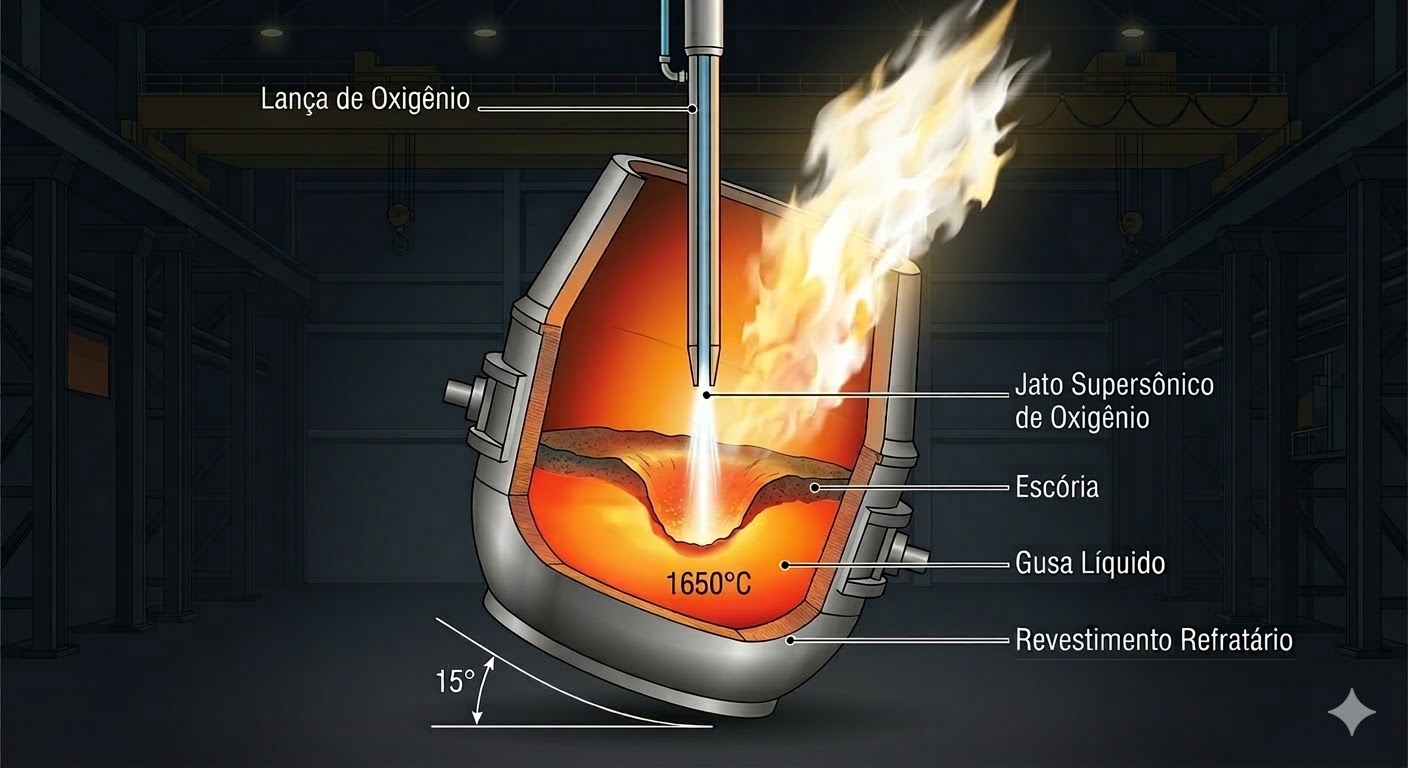
\includegraphics[width=0.55\textwidth]{Images/BOF_Illustration}
\caption{Seção transversal de um BOF (Forno a Oxigênio Básico). Lança de O\textsubscript{2}, escória, gusa líquido e revestimento refratário. (Nano Banana Pro~3.)}
\label{fig:bof}
\end{figure}

\textbf{Variáveis monitoradas e alvos de qualidade.}
O acerto simultâneo da temperatura final ($T_\text{final}=1650\pm10$\,°C) e do teor de carbono residual ($0{,}03$–$0{,}08$\,\%) é crítico: esses dois parâmetros definem a eficiência de dessulfuração subsequente e a estabilidade do vazamento contínuo\,\cite{wang2020endpoint,diaz2019hotmetaltemp}. Modelos de ML com atributos tabulares amplos aplicados a dados reais de planta já reportam MAE de temperatura da ordem de $8\,^\circ\text{C}$ e de carbono da ordem de $7\times10^{-3}\,\%$~em~massa\,\cite{zhou2024bof} --- valores mais rigorosos do que os limiares de $10\,^\circ\text{C}$ e $0{,}020\,\%$ adotados nesta dissertação (Seção~\ref{sec:objetivo}); a diferença reflete o uso de dados reais de planta e de um conjunto de atributos tabulares mais amplo do que o desta dissertação, não uma meta menos ambiciosa (Seção~\ref{sec:comparacao-literatura}, Capítulo~\ref{chp:resultados}). Além de C, Si e Mn, monitoram-se P, S, Cr, Ni e Cu, bem como Fe e O dissolvidos; o potencial redox de cada espécie compete pelo oxigênio disponível, e conhecer essas interações é essencial para dosar fluxantes e otimizar o perfil de sopro\,\cite{bae2020bof}.

\textbf{Balanços estequiométrico e entálpico.}
Antes do sopro, balanços de massa determinam a quantidade de sucata, cal e oxigênio necessária para as reações principais:
\[
\text{C + O}_2 \rightarrow \text{CO}_x,\quad
\text{Si + O}_2 \rightarrow \text{SiO}_2,\quad
\text{Mn + O}_2 \rightarrow \text{MnO},
\]
enquanto um balanço de entalpia calcula que aproximadamente 65\,\% do calor total provém do calor sensível do gusa e 35\,\% do ganho exotérmico das oxidações\,\cite{madhavan2020heatbalance}. Esses cálculos definem a janela de sucata que pode ser fundida sem comprometer a temperatura alvo e a fração ótima de fluxantes. A explicitação desses balanços como atributos de entrada de modelos de ML — em vez de deixá-los implícitos nos dados brutos — é o princípio central da engenharia de atributos físico-derivados adotada nesta dissertação.

\textbf{Integração sensor–modelo.}
A Figura~\ref{fig:bof-process-flow} sintetiza as sete etapas operacionais do sopro, do carregamento do metal líquido à escorificação final. Sinais brutos de termopares, medidores de vazão e espectrômetros são filtrados e temporalmente alinhados para gerar variáveis derivadas — massa oxidada, excedente de entalpia, eficiência de uso de O\textsubscript{2} — que condensam relações não-lineares de difícil aprendizado direto\,\cite{willard2020integrating}, conforme ilustrado na Figura~\ref{fig:bof-process-diagram}. Tais atributos alimentam modelos híbridos que refinam a estimativa do \emph{endpoint} em tempo quase real\,\cite{chattopadhyay2022hybrid,xia2024dmpinn}, reduzindo a necessidade de amostragens manuais e melhorando a robustez operacional em condições de carga variável.

\begin{figure}[htbp]
\centering
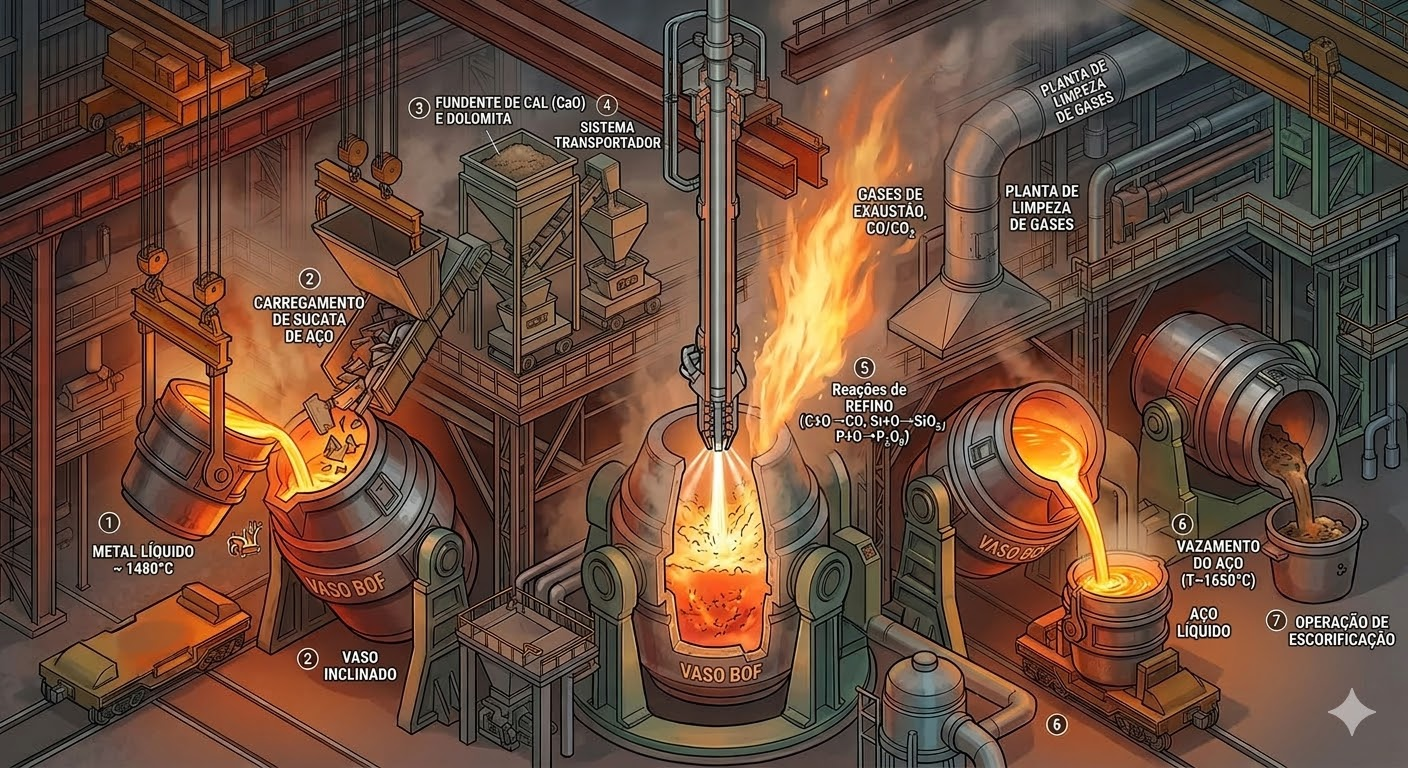
\includegraphics[width=0.82\textwidth]{Images/FLuxo_BOF}
\caption{Fluxo operacional completo do processo BOF: (1)~carregamento do metal líquido ($\approx\!1480$\,°C), (2)~inclinação do vaso, (3)~adição de fundentes (CaO, dolomita) via sistema transportador, (4)~sopro de O\textsubscript{2} com reações de refino, (5)~exaustão e limpeza de gases CO/CO\textsubscript{2}, (6)~vazamento do aço líquido e (7)~escorificação. Ilustração gerada com auxílio de inteligência artificial (Nano Banana Pro~3).}
\label{fig:bof-process-flow}
\end{figure}

\begin{figure}[htbp]
\centering
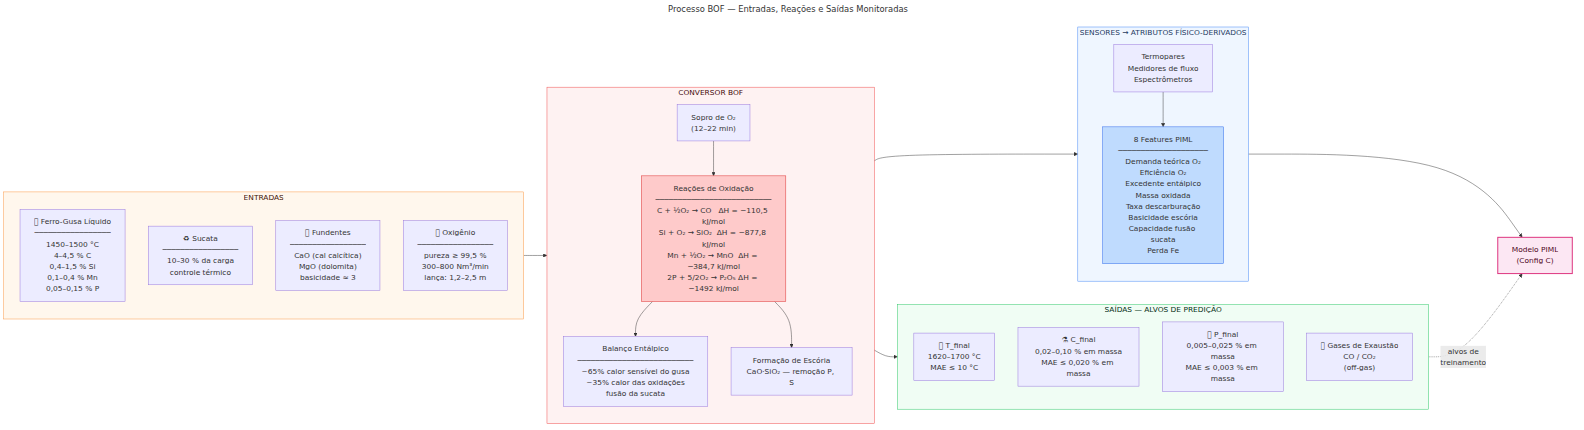
\includegraphics[width=0.82\textwidth]{Images/diagrams/05_bof_process}
\caption{Diagrama esquemático do processo BOF: entradas (gusa líquido, sucata, fundentes e O\textsubscript{2}), reações de oxidação no conversor, saídas monitoradas (T\textsubscript{final}, C\textsubscript{final}, P\textsubscript{final}) e derivação dos oito atributos físico-derivados a partir dos sinais de sensores para o modelo PIML.}
\label{fig:bof-process-diagram}
\end{figure}

Em conclusão, tem-se que compreender a natureza, estequiometria e entalpia dos insumos --- gusa, sucata, fluxantes e oxigênio --- é decisivo para atingir temperatura e composição alvo na primeira tentativa. A hipótese central desta dissertação (Seção~\ref{sec:objetivo}) é que a inclusão explícita desses balanços nos atributos do modelo melhora o erro preditivo além de fornecer explicações físico-químicas potencialmente mais transparentes; o Capítulo~\ref{chp:resultados} avalia essa hipótese empiricamente, com resultado dependente do alvo de predição.

%-------------------------------------------------------------------%
\section{Geração de Dados Sintéticos para Processos Industriais}
\label{sec:dados-sinteticos-fund}

Dados rotulados de processos industriais são escassos por razões práticas: cada corrida em um BOF ou ciclo de um EAF representa custo elevado de energia e materiais, e a coleta de rótulos precisos (composição química final, temperatura) exige análise laboratorial ou sensores especializados\,\cite{buggineni2024synthetic}. Essa escassez motiva o uso de dados sintéticos gerados por modelos físico-matemáticos como substitutos para o treinamento de modelos de ML.

A literatura sobre dados sintéticos tabulares distingue quatro categorias de métodos de geração: amostragem paramétrica (Monte Carlo e variantes), modelos baseados em cópulas, redes generativas adversariais (GANs) e autoencoders variacionais (VAEs)\,\cite{buggineni2024synthetic,melo2024synthetic}. Para processos industriais cujas restrições físicas são bem conhecidas e o tamanho amostral alvo é da ordem de milhares — não milhões —, a amostragem Monte Carlo com validação por balanço de massa ou energia é mais transparente, reproducível e computacionalmente econômica do que abordagens generativas profundas\,\cite{buggineni2024synthetic,morales2025synthetic}.

A validade dos dados sintéticos depende de dois requisitos: (i) as faixas de amostragem devem cobrir o espaço operacional real do processo, derivadas de fontes industriais ou literatura especializada; e (ii) cada instância gerada deve satisfazer as leis de conservação pertinentes, descartando-se amostras fisicamente implausíveis\,\cite{buggineni2024synthetic,melo2024synthetic}. \citeauthor{melo2024synthetic} demonstraram que dados sintéticos gerados sob essas condições produzem modelos de ML com desempenho comparável aos treinados em dados reais para tarefas de regressão de processo em gêmeos digitais industriais\,\cite{melo2024synthetic}. \citeauthor{morales2025synthetic} confirmaram resultado análogo para manutenção preditiva, concluindo que dados sintéticos fisicamente coerentes permitem generalização adequada desde que as distribuições marginais e as correlações relevantes do processo sejam preservadas\,\cite{morales2025synthetic}.

Uma limitação inerente à abordagem sintética é que os modelos treinados aprendem a estrutura imposta pelo gerador, não necessariamente a do processo real. Portanto, métricas de desempenho obtidas em dados sintéticos devem ser interpretadas como evidências de viabilidade metodológica, não como estimativas de performance em planta\,\cite{giannini2022synthetic}. A validação em dados reais é etapa obrigatória antes de qualquer implantação industrial.

%-------------------------------------------------------------------%
\section{Interpretabilidade em Modelos de ML Industrial}
\label{sec:interpretabilidade}

Modelos de aprendizado de máquina de alta capacidade — como Random Forest, XGBoost e redes neurais profundas — atingem baixo erro preditivo em muitos problemas industriais, mas permanecem como caixas-pretas do ponto de vista do operador de processo\,\cite{inglis2022visualisation}. A interpretabilidade é essencial nesse contexto por duas razões: (i) permite validar se o modelo capturou relações fisicamente coerentes, e não correlações espúrias presentes nos dados de treinamento; e (ii) aumenta a confiança e a aceitação pelos profissionais que devem tomar decisões com base nas predições\,\cite{inglis2022visualisation,manojlovic2022eaf}.

Entre os métodos de interpretabilidade disponíveis, destacam-se três abordagens principais: importância por permutação, \textit{Integrated Gradients} e SHAP. A importância por permutação mede o aumento do erro ao embaralhar aleatoriamente os valores de um atributo, sendo simples e agnóstica ao modelo, porém sensível a correlações entre atributos e incapaz de fornecer explicações por instância\,\cite{inglis2022visualisation}. \textit{Integrated Gradients} oferece explicações locais baseadas em gradientes, sendo restrito a modelos diferenciáveis e, portanto, inaplicável a modelos de árvore\,\cite{inglis2022visualisation}. O método SHAP (\textit{SHapley Additive exPlanations}), fundamentado na teoria de jogos cooperativos, atribui a cada atributo uma contribuição marginal para a predição de cada instância\,\cite{lundberg2017unified}. Ao contrário de medidas de importância globais (como a impureza média em Random Forests), SHAP fornece explicações locais — por instância — e é consistente: se um atributo se torna mais importante, seu valor SHAP aumenta. Para esta dissertação, SHAP é a escolha natural por três razões: (i) é agnóstico ao algoritmo, aplicando-se igualmente a modelos lineares, Random Forest, XGBoost e MLP; (ii) fornece explicações locais com garantias axiomáticas de consistência e eficiência; e (iii) possui implementações eficientes (\texttt{TreeExplainer}) que tornam sua aplicação computacionalmente viável para os modelos de ensemble avaliados. \citeauthor{manojlovic2022eaf} aplicaram SHAP a modelos de eficiência energética em EAF e demonstraram que os atributos com maior importância SHAP correspondiam às variáveis operacionais que especialistas de processo já identificavam como determinantes — uso de oxigênio e peso de corrida —, validando a coerência física do modelo\,\cite{manojlovic2022eaf}.

Para o contexto desta dissertação, a análise SHAP serve como mecanismo de validação físico-informada: espera-se que atributos derivados de balanços de massa e energia (\texttt{theo\_o2\_demand}, \texttt{enthalpy\_surplus}, \texttt{slag\_basicity}) apresentem alta importância nos modelos treinados com a configuração físico-informada (Config~C), e que as direções de influência correspondam ao comportamento esperado pela termodinâmica\,\cite{manojlovic2022eaf,xia2024dmpinn}. Por exemplo, \texttt{slag\_basicity} deve influenciar positivamente a remoção de fósforo: maior basicidade favorece a oxidação de P para a escória\,\cite{bae2020bof}.

%-------------------------------------------------------------------%
\section{Arquiteturas Híbridas Físico-Informadas}
\label{sec:arquiteturas-hibridas}

A literatura identifica três topologias principais para integrar modelos físicos e de ML em sistemas híbridos, ilustradas na Figura~\ref{fig:hybrid-architectures}\,\cite{chattopadhyay2022hybrid,willard2020integrating}. Na arquitetura \textbf{serial}, modelo físico e modelo de ML trocam informação em múltiplas etapas de um mesmo pipeline, com a saída de um alimentando a entrada do outro; \citeauthor{chattopadhyay2022hybrid} adotam essa topologia em BOF, com modelos termodinâmicos de balanço de entalpia e oxigênio fornecendo estimativas iniciais e redes neurais treinadas nas variáveis brutas realimentando suas predições de volta aos modelos teóricos (Capítulo~\ref{chp:capitulo3})\,\cite{chattopadhyay2022hybrid}. Na arquitetura \textbf{paralela}, as saídas do modelo físico e do modelo de ML são combinadas por uma camada de fusão que aprende pesos adaptativos; \citeauthor{shao2024hybrid} utilizam estrutura análoga para predição do tempo de sopro\,\cite{shao2024hybrid}.

A terceira topologia — \textbf{informada por atributos} — não exige que o componente físico seja diferenciável nem que faça parte do grafo computacional do modelo de ML. Em vez disso, grandezas calculadas por modelos físicos (balanços de massa, energia, estequiometria) são incorporadas como variáveis de entrada adicionais\,\cite{willard2020integrating}. Essa abordagem é compatível com qualquer algoritmo de ML e impõe o menor custo de implementação, sendo vantajosa quando o componente físico não precisa ser diferenciável e quando a integração deve ser feita de forma agnóstica ao algoritmo de aprendizado\,\cite{willard2020integrating}.

O \textit{framework} físico-informado de \citeauthor{wang2025phoenix} para soldagem robótica, publicado na \textit{Nature Communications}, demonstra a escalabilidade da abordagem informada por atributos para processos de manufatura de alta complexidade, obtendo ganhos expressivos em relação a linhas de base puramente orientadas a dados e a modelos físicos puros\,\cite{wang2025phoenix}. Esses resultados reforçam a escolha metodológica desta dissertação: a Config~C implementa a topologia informada por atributos, calculando os oito atributos físico-derivados definidos na Seção~\ref{subsec:feature-engineering} e incorporando-os ao conjunto de features de todos os modelos avaliados.

\begin{figure}[htbp]
\centering
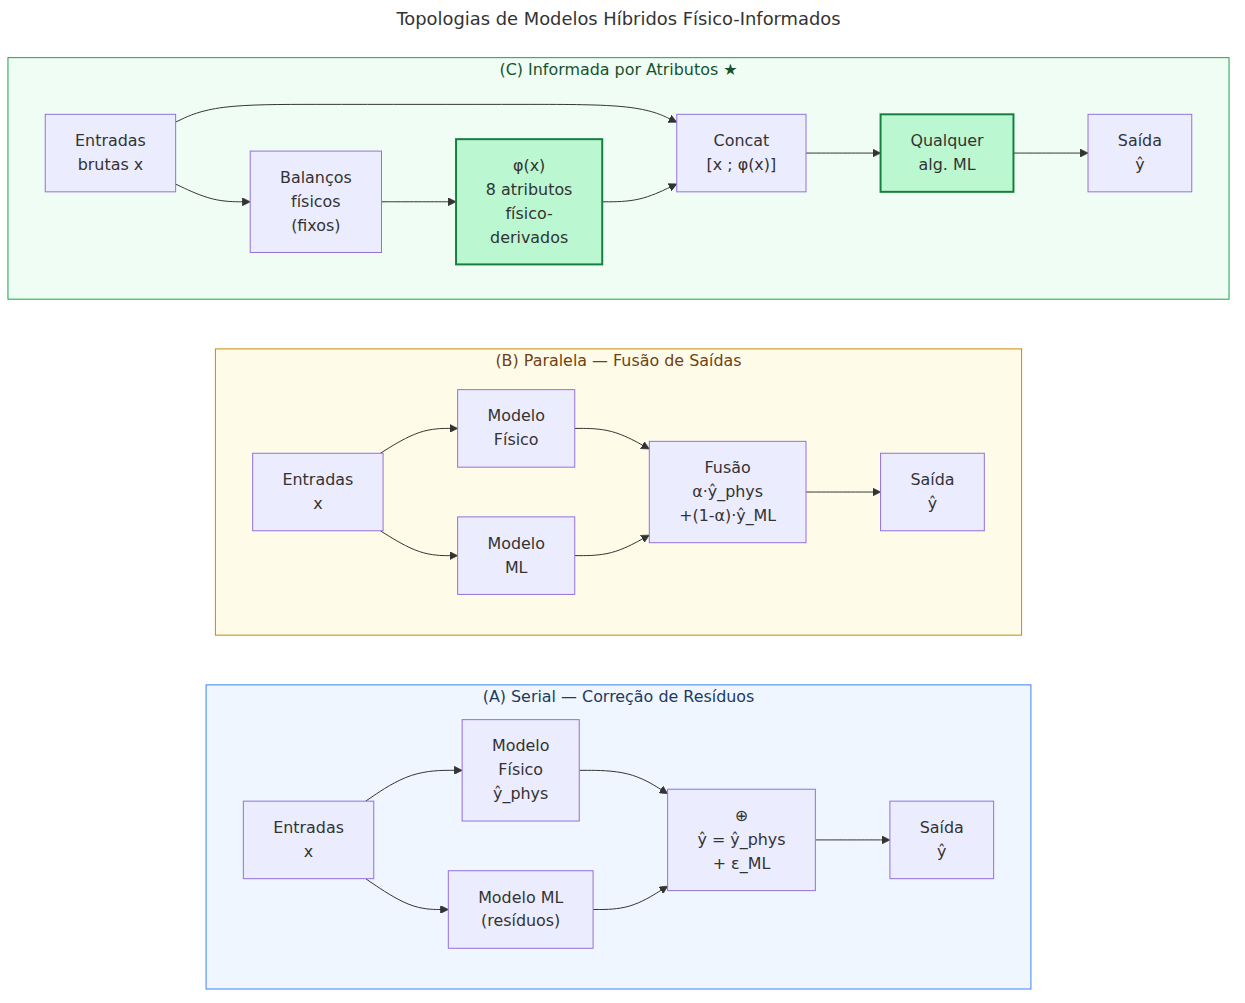
\includegraphics[width=0.78\textwidth,height=0.28\textheight,keepaspectratio]{Images/diagrams/03_hybrid_architectures}
\caption{Topologias de modelos híbridos físico-informados: (A)~serial com correção de resíduos, (B)~paralela com camada de fusão e (C)~informada por atributos — arquitetura adotada nesta dissertação. Adaptado de \,\cite{willard2020integrating}.}
\label{fig:hybrid-architectures}
\end{figure}